\documentclass{article}
\usepackage{exercise}
\usepackage[obeyspaces]{url}
\usepackage[dvipsnames]{xcolor}
\usepackage{graphicx}
\usepackage{listings}
\usepackage[scaled]{helvet}
\usepackage{amsmath,amssymb,amsfonts,mathtools,cancel}

% typeset in helvetica
\renewcommand*\familydefault{\sfdefault}


% QE stuff
\def\qe{{\sc Quantum ESPRESSO}}
\def\pwx{\texttt{pw.x}}
\def\cpx{\texttt{cp.x}}
\def\phx{\texttt{ph.x}}
\def\nebx{\texttt{neb.x}}
\def\configure{\texttt{configure}}
\def\PWscf{\texttt{PWscf }}
\def\PHonon{\texttt{PHonon}}
\def\CP{\texttt{CP}}
\def\PostProc{\texttt{PostProc}}
\def\NEB{\texttt{PWneb}} % to be decided
\def\make{\texttt{make}}
%%%%%%%%%%%%%%%%%%%%%%%%

\def\ipi{i-PI}
\newcommand{\hints}[1]{\emph{Hints: #1}}
\newcommand{\lstinxml}{\lstinline[language=XML]}
\newcommand{\lstinbash}{\lstinline[language=Bash]}
\usepackage[space=true]{accsupp}

\newcommand{\pdfactualhex}[3]{\newcommand{#1}{%
\BeginAccSupp{method=hex,ActualText=#2}#3\EndAccSupp{}}}

% PASTABLE lstlisting code
\pdfactualhex{\pdfactualdspace}{2020}{\textperiodcentered\textperiodcentered}
\pdfactualhex{\pdfactualsquote}{27}{'}
\pdfactualhex{\pdfactualbtick}{60}{`}

\lstset{tabsize=4,basicstyle=\ttfamily,breaklines=true,columns=flexible,emptylines=10000}
\lstset{literate={'}{\pdfactualsquote}1
                 {`}{\pdfactualbtick}1
                 {\ \ }{\pdfactualdspace}2
}

\lstset{
    basicstyle=\ttfamily,
    keywordstyle=\color{BrickRed},
    commentstyle=\color{Gray},
    stringstyle=\color{black},
    emphstyle=\color{RedOrange},
    columns=flexible,
    showstringspaces=false,
    xleftmargin=1em,
    deletekeywords={bin,all}
}


\lstdefinelanguage{Bash}
{
   alsodigit={-,.},
   morekeywords={ cp2k.popt, lmp_ubuntu, i-pi, vmd, for, done, python, mpirun, touch, tail, trajworks, autocorr, awk, i-pi-mergebeadspdb, grep, head, cp, cd, cat, ls, pwd, bash, sed, mkdir, vi, sh}
   %morecomment=[s][\color{orange}]{#}{\}
}

%\lstdefinelanguage{Python}
%{
%    morecomment=[s][\color{orange}]{#}{\}
%}


\lstdefinelanguage{XML}
{
  morestring=[b][\color{RedOrange}]",
%  morestring=[s]{>}{<},
  morecomment=[s]{<?}{?>},
  morecomment=[s][\color{orange}]{<!--}{-->},
  identifierstyle=\color{BlueViolet},
  keywordstyle=\color{ForestGreen},
  stringstyle=\color{RedOrange},
%  tagstyle=\color{Blue},
  morekeywords={xmlns,version,type, mode, units, forcefield, filename, stride, overwrite, nbeads,prefix}% list your attributes here
}

\lstdefinestyle{XML}
{
\tagstyle=\color{Blue}
}

\title{An introduction to path integral \\molecular dynamics using \ipi{}}
\author{Venkat Kapil}
\date{June 2016}

\setlength\parindent{0pt}
\begin{document}
\maketitle

% INTRO
In this set of exercises we will learn about the basics of doing (path integral) molecular dynamics simulations using \ipi{}. We will begin by performing conventional molecular dynamics simulation of classical nuclei, and move towards highly quantum mechanical systems. In the process, the design principles, features and input/output format of \ipi{} will be introduced.

\begin{Exercise}[label={i-pi},title={Molecular Dynamics: a client/server approach}]

We will start by providing a basic introduction to molecular dynamics. Under the Born-Oppenheimer approximation, the dynamics of the electronic degrees of freedom is completely decoupled from that of the nuclei; the electrons always occupy the ground state for each configuration of the nuclei. The electronic degrees of freedom are averaged out to an effective potential that is felt by the nuclei. This is called the Born-Oppenheimer potential and can be either computed by solving the Schr\"odinger equation or be approximated by a classical force field. In a fully classical treatment of nuclei, the additional assumption is made that their dynamics can be described in terms of the Hamiltonian:
\begin{eqnarray}
    H(\textbf{p},\textbf{q})=\sum_i \dfrac{\textbf{p}_i^2}{2 m_i} + V(\{\textbf{q}_i\}),
\end{eqnarray}
where $m_i$, $\textbf{p}_i$ and $\textbf{q}_i$ are the mass, the momentum and the coordinates of the $i$-th nucleus, respectively and $V(\{\textbf{q}_i\})$ is the  Born-Oppenheimer potential. In order to simulate the time evolution of nuclei the following equations of motion have to be integrated:
\begin{eqnarray}
   \dfrac{d \textbf{p}_i}{d t}&=& 
   - \dfrac{\partial H(\textbf{p},\textbf{q})}{\partial \textbf{q}_i}=-\frac{d V(\{\textbf{q}_i\})}{d\textbf{q}_i} \\
   \dfrac{d \textbf{q}_i}{d t}&=& 
   + \dfrac{\partial H(\textbf{p},\textbf{q})}{\partial \textbf{p}_i} = + \frac{\textbf{p}_i}{m_i}.
\end{eqnarray}
\begin{figure}[h]
    \begin{center}
    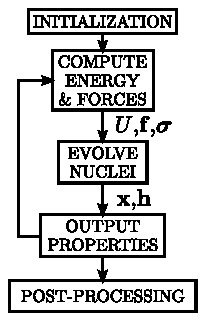
\includegraphics[width=0.25\textwidth]{mdchart.pdf}
    \end{center}
    \caption{At the initialization stage, the program is informed about some basic information about the system, such as the number of atoms, their types, system size, etc. and the initial position and momentum. After that, the program goes through the loop Forces $\rightarrow$ Motion $\rightarrow$ Analysis once per discrete simulation time step. The force acting on each atom is evaluated first, and are then used to advance the momenta and the coordinates of the nucleus. At the analysis step, the properties of interest for the system can be computed, stored, or analyzed on the fly.
    \label{fig:MD_flow}}
\end{figure}

The key processes of a molecular dynamics run are illustrated in the flowchart in figure \ref{fig:MD_flow}. From the flowchart above, one can observe that each block of the program can be easily modularized.
One can, for example, carry out the force evaluation using one program, and only communicate the results to another program which performs the motion and the analysis parts. This is precisely the philosophy behind i-PI, which acts as a server that takes care of the evolution of nuclei and the evaluation of properties of the system, having as clients other programs that compute forces and potential energies. An graphical representation of how \ipi{} works is given in the scheme below.

{\centering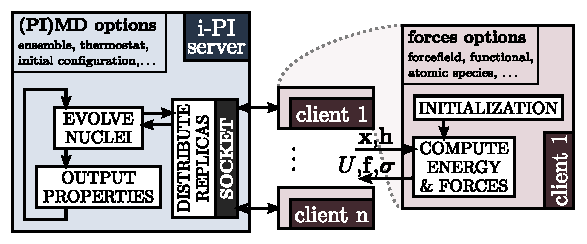
\includegraphics[width=0.9\textwidth]{ipi-scheme.pdf}} \\



In this exercise, we will perform a simple Molecular Dynamics (MD) calculation for gas phase water. Instead of doing the simulation directly using an out-of-the-box MD software such as CP2K~\cite{citeCP2K}, we are going to complete the task in a slightly twisted manner. We are going to use i-PI in conjunction with CP2K to demonstrate a client/server model for (path integral) molecular dynamics as well as the subtle advantages that it brings. The simulation will be performed on one gas phase water molecule using the $NVT$ ensemble at 300K. We will also record the kinetic and potential energy of the system.

\Question
Read the CP2K input file \url{ex-1/cp2k.in}. The specifications:
\begin{lstlisting}[language=bash]
&XC_FUNCTIONAL BLYP
&END XC_FUNCTIONAL
...
...
&KIND O
BASIS_SET DZVP-GTH
POTENTIAL GTH-BLYP-q6
&END KIND

\end{lstlisting}
means that the BLYP exchange functional is being used while the core electrons are being replaced by the Goedecker-Teter-Hutter pseudopotential. 

In the part of the input file that specifies how to integrate the
equations of motion, this line:
\begin{lstlisting}[language=bash]
&MOTION
&DRIVER
HOST drivercp2k
UNIX TRUE
PORT 20614
&END DRIVER
&END MOTION
\end{lstlisting}
is used, which basically means CP2K will only be in charge of the 
force evaluation and send that information to \ipi{}.
The latter will take care of the motion and the analysis parts.
All the information will be transmitted through a UNIX-domain socket with the name \url{drivercp2k}, which is a mechanism for local, inter-process communication.

\Question
Now open the \ipi{} input file \url{input.xml} in the same folder.
For a moment let us ignore all the other entries but only focus on the followings
\begin{lstlisting}[language=xml]
 <ffsocket mode="unix" name="cp2k">
 <address> drivercp2k </address>
 </ffsocket>
\end{lstlisting}
This indicates that \ipi{} will receive any information sent by LAMMPS through the UNIX-domain socket with the tag \url{drivercp2k},
and send the coordinates of the nuclei in the system to LAMMPS for force evaluations using the same socket.

\Question
Let"s run an \ipi{}+CP2K Molecular Dynamics simulation!
Open a terminal at the current directory and
launch \ipi{} by typing
\begin{lstlisting}[language=bash]
$ i-pi input.xml 
\end{lstlisting}
At this point \ipi{} should start 
%and show a logo like this
%\begin{figure}[h]
%\centering
%    
\includegraphics[width=0.2\textwidth]{ipi-logo.pdf}
%\end{figure}
and parse the input file. At the bottom of the output on the screen it should say
\begin{lstlisting}[language=bash]
Created unix socket with address drivercp2k
@ForceField: Starting the polling thread main loop.
\end{lstlisting}
This means \ipi{} has started properly, has created the UNIX socket, and is waiting for the communications from the clients that do force evaluations.

\Question
Now is a good time to start CP2K. Open up a second terminal either manually or by typing \url{Ctrl+Shift+t} and start CP2K by entering the command
\begin{lstlisting}[language=bash]
$ cp2k.popt -i cp2k.in
\end{lstlisting}
Then CP2K should start and dump out some outputs.

\Question
Now switch to the terminal where \ipi{} is running, notice that \ipi{} has built the connection with LAMMPS with the message
\begin{lstlisting}[language=sh]
 @SOCKET:   Client asked for connection from . Now hand-shaking.
 @SOCKET:   Handshaking was successful. Added to the client list.
\end{lstlisting}
and started the Molecular Dynamics simulation.
It should also dump out information on the time cost of each MD step.

\Question
What we are going to do now is to kill CP2K.
Simply switch to the terminal where CP2K is running and press \url{Ctrl+c}.
Now look at whether \ipi{} is still running.
Notice that although the evolution of MD is paused, \ipi{} itself does not die off but instead continue to run and wait for new client to take over.
Now start CP2K again by typing
\begin{lstlisting}[language=bash]
$ cp2k.popt -i cp2k.in
\end{lstlisting}
What happens to \ipi{} now?

\Question
What if one stops \ipi{}? 
Kill \ipi{} by typing \url{Ctrl+c} where it is running, or create a file named \url{EXIT} in the folder where \ipi{} is running
(you can use the bash command \url{touch EXIT}).
Watch how \ipi{} responds, and how CP2K reacts.
Think about what are the advantages of a clean exit when a MD program stops unexpectedly.

\Question
Take a look at all the output files dumped by \ipi{}.
You should have \url{simulation.out} that describe the system properties,
\url{simulation.pos_0.pdb} that records the atomic trajectories,
and \url{RESTART} that contains all the information to restart the simulation. 
\end{Exercise}

\begin{Exercise}[label={inputs},title={Keywords, outputs, and units of \ipi{}}]
\noindent In this exercise we are going to familiarize ourselves with the important notations of \ipi{} input files. We will stick with the same system but we will perform a $32$ beads path integral molecular dynamics simulation. 

\Question
Let"s take a close look at the units first - which are the source of many errors during simulation and analysis.
All the units used internally by \ipi{} are atomic units, as given
below.

\texttt{
\begin{center}
\begin{tabular}{lll}
\hline\hline
Unit & Name & S.I. Value\\
\hline 
Length & Bohr radius & 5.2917721e-11 m\\
Time & N.A. & 2.4188843e-17 s\\
Mass & Electron mass & 9.1093819e-31 kg\\
Temperature & Hartree & 315774.66 K\\
Energy & Hartree & 4.3597438e-18 J\\
Pressure & N.A. & 2.9421912e13 Pa\\
\hline\hline
\end{tabular}
%\par\end{center}
\end{center}
}

By default, both input and output data are given in atomic
units, but in most cases the default units can be overridden if one
wishes so. 
For example, in \url{ex-2/input.xml}
we used
\begin{lstlisting}[language=xml]
<properties stride="1" filename="out">
[ step, time{picosecond}, conserved, temperature{kelvin}, kinetic_cv, potential ]
</properties>
<trajectory filename="pos" format="pdb" stride="1"> positions {angstrom} </trajectory>
\end{lstlisting}
so that the time, temperature, and the trajectory will written out in the units of picosecond, Kelvin, and Angstrom in the output files, respectively. Similarly, the units of the initialization files can be specified such as
\begin{lstlisting}[language=xml]
<cell mode="abc" units="angstrom"> [ 8, 8, 8 ] </cell>
<velocities mode="thermal" units="kelvin"> 300 </velocities>
\end{lstlisting}
Note that the units of the xyz file have to be specified in the comment line:
\begin{lstlisting}[language=xml]
3
# positions{angstrom}
 O 0.54044984 -0.97485007 -0.21657970
 H 1.74328720 -0.90927800 -0.10039502
 H 0.18385954 -1.25804198 -1.07875142
\end{lstlisting}
When using \ipi{}, you can play around with the units to facilitate the initialization process as well as subsequent analyses. 

\Question
Now we will observe the format and structure of \url{input.xml}.
The xml file consists of a set of hierarchically nested tags. There are three
parts to an xml tag. Each tag is identified by a tag name, which specifies the class
or variable that is being initialized. Between the opening and closing tags there is some data, 
which is used to specify the
contents of a class object, or the value of a variable. Finally tags can have attributes,
which are used to specify how the tag should be interpreted.
A xml tag has the following syntax:
\begin{lstlisting}[language=xml]
<tag_name attrib_name=attrib_data>tag_data</tag_name>
\end{lstlisting}
For example, in the tag
\begin{lstlisting}[language=xml]
<thermostat mode="pile_l">
<tau units="femtosecond">100</tau> 
<pile_lambda>0.1</pile_lambda>
</thermostat>
\end{lstlisting}
the tag name \lstinxml{thermostat} indicates which part of the simulation options is being defined,
\lstinxml{mode="pile_l"} specifies the type of thermostat in use,
and \lstinxml{<tau units="femtosecond">100</tau>} is used to set the parameters used for this particular thermostat.
Please browse around this \url{input.xml} to see if you can make sense of most of the attributes.

\Question
It is worth spending a bit more time to explain about the type of socket used here.
For the communication between \ipi{} and client codes, both Internet and Unix domain sockets can be used: the
latter allow for fast communication on a single node, whereas the former make it possible
to run \ipi{} and the clients on different computers.
Here we demostate how to use the Internet (TCP/IP) sockets.
In \ipi{} input file we have
\begin{lstlisting}[language=xml]
<ffsocket mode="inet" name="cp2k">
<latency> 1.00e-02</latency>
<slots> 4 </slots>
<port> 20614 </port>
<timeout> 6.00000000e+02 </timeout>
<address> localhost </address>
</ffsocket> 
\end{lstlisting}
and in CP2K input file \url{cp2k.in} we have the following
\begin{lstlisting}[language=bash]
&MOTION
&DRIVER
HOST localhost
PORT 20614
&END DRIVER
&END MOTION
\end{lstlisting}
The above means that an Internet domain socket with port number 20614 is used for the communication.
The port number is an integer between 1 and 32767 used to distinguish between all the
different sockets open on a particular host. As many of the lower numbers are reserved
for use in important system processes or Internet communication, it is generally advisable
to only use numbers in the range 1025-32767 for simulations.

\Question
Now let"s see whether the Internet domain socket can indeed connect. But before that make the necessary changes in the input files as indicated by the comments. 
Type the following to start \ipi{} and CP2K:
\begin{lstlisting}[language=bash]
$ i-pi input.xml &> log.ipi &
$ cp2k.popt -o h2o.out cp2k.in &
\end{lstlisting}
Does it work? If you have access to two computers that can communicate with each
other on the same network, you can try to run in a distributed-computing mode,
with i-PI running on one computer and CP2K on the other. This advanced mode of 
operation, however, can be complex in the presence of firewalls or multiple 
network interfaces (see the i-PI documentation for some examples). 

\end{Exercise}

\begin{Exercise}[label={water},title={Multiple time steps with an \emph{ab initio} potential}]
In this exercise we will perform a PIMD simulation  with multiple time steps in real and imaginary time, so that it becomes cheap enough to run it on your laptops. The main idea is to find a cheap potential that captures the quickly-varying components of the physical potential. This way the potential can be split into:
\begin{align*}
    V(\{\textbf{q}_i\}) = V^{\text{cheap}}(\{\textbf{q}_i\}) + [V(\{\textbf{q}_i\}) - V^{\text{cheap}}(\{\textbf{q}_i\})]
\end{align*}
Since the cheap potential is a good approximation to the fast components, the difference potential should be slowly varying which can be integrated with a larger time step and be computed on a smaller ring polymer (or in the best case scenario the centroid).
\begin{align*}
    \sum_{j=0}^{P-1} V(\{\textbf{q}_i^{(j)}\}) & = \sum_{j=0}^{P-1} V^{\text{cheap}}(\{\textbf{q}_i^{(j)}\}) + \sum_{j=0}^{P-1} [V(\{\textbf{q}_i^{(j)}\}) - V^{\text{cheap}}(\{\textbf{q}_i^{(j)}\})] \\
    & \approx \sum_{j=0}^{P-1} V^{\text{cheap}}(\{\textbf{q}_i^{(j)}\}) +  P [V(\{\textbf{q}_i^{(0)}\}) - V^{\text{cheap}}(\{\textbf{q}_i^{(0)}\})]
\end{align*}

\Question
Enter the directory \url{ex-4/} and look at the \ipi{} input. You should find the following lines:
\begin{lstlisting}[language=xml]
<ffsocket mode="unix" name="qt32">
<latency> 1.00000000e-04 </latency>
<address> driverqt32 </address>
</ffsocket>
<ffsocket mode="unix" name="qt01">
<latency> 1.00000000e-04 </latency>
<address> driverqt01 </address>
</ffsocket>
\end{lstlisting}
It has specified two additional force providers called \lstinbash{qt32} and \lstinbash{qt01} associated with two unix sockets called \lstinbash{driverqt32} and \lstinbash{driverqt01}. Now look at the \lstinxml{<forces></forces>} section:
\begin{lstlisting}[language=xml]
<forces>
<force forcefield="cp2k" nbeads="01">
<mts_weights> [1, 0] </mts_weights>
</force>
<force forcefield="qt32" nbeads="32">
<mts_weights> [0, 1] </mts_weights>
</force>
<force forcefield="qt01" nbeads="01">
<mts_weights> [-1, 0] </mts_weights>
</force>
</forces>
\end{lstlisting}
It shows that the force components associated with the \lstinbash{qt01} and \lstinbash{cp2k} force providers will be computed on 1 bead while the ones associated with \lstinbash{qt32} will be computed on 32 beads. The \lstinxml{<mts_weights></mts_weights>} allows one to represent the forces computed at various MTS levels as a linear combination of the components. It is a vector that represents the weight of a force at all the MTS levels (starting from the outer). This mean that the force that will be integrated in the outer and inner MTS loops are:
\begin{align*}
    & V^{\text{outer}} = V^{\text{cp2k}} - V^{\text{qt01}} \\
    & V^{\text{inner}} = V^{\text{qt32}}
\end{align*}

\Question
Observe the \lstinxml$<initialize></initialize>$ section. We will be initializing from a checkpoint file 
\lstinbash{init.chk} which is basically a RESTART file of a long equilibration run. 
For a PIMD simulation, we will set \lstinbash{nbeads} to $32$ as against $1$ for a classical simulation.

\begin{lstlisting}[language=xml]
<initialize nbeads="32">  
<file mode="chk"> init.chk </file>
</initialize>
\end{lstlisting}

\Question
Look at  the \lstinxml{dynamics} part of the \lstinxml{<motion></motion>} section:
\begin{lstlisting}[language=xml]
<dynamics mode="mts">
<timestep units="femtosecond"> 1.00 </timestep>
<thermostat mode="pile_l">
<tau units="femtosecond"> 100 </tau>
<pile_lambda> 0.1 </pile_lambda>
</thermostat>
<nmts> [1,4] </nmts>
</dynamics>
\end{lstlisting}
We shall be using the \lstinbash{mts} integrator with \lstinxml{<nmts> [1,4] </nmts>} indicates the number of epocs in the outer and inner MTS loops. Consequently, the inner part will be integrated with a time step of $1/4 = 0.25$ fs  while the outer part will be integrated with a time step of $1$ fs.

\Question
To run the simulation launch \ipi{} and CP2K in background, it is advisable to keep  separate logs:
\begin{lstlisting}[language=bash]
$ i-pi input.xml &> log.i-pi &
$ cp2k.popt -i cp2k.in > log.cp2k & 
\end{lstlisting}
For the cheap potential we will use the qtip4pf water potential, which so happens to be implemented in an \ipi{} driver. To run the driver use:
\begin{lstlisting}[language=bash]
$ i-pi-driver -u -h qt01 -m qtip4pf &> log.qt01 &
$ i-pi-driver -u -h qt32 -m qtip4pf &> log.qt32 &
\end{lstlisting}
At this point wait for a few tens of steps. You can monitor the conserved quantity and the centroid virial kinetic energy by plotting the third  and the fifth columns of the output file.
\begin{lstlisting}[language=bash]
$ p "simulation.out" u 1:3 w l, "" us 1:5 w l
\end{lstlisting}
\Question
In order to visualize the ring polymer you can run the i-pi-mergebeadspdb tool that takes the position of all the beads and returns one pdb output with a ring polymer for each atom.
\begin{lstlisting}[language=bash]
$ i-pi-mergebeadspdb simulation pos > simulation-all.pdb 
\end{lstlisting}
Use VMD to vistalize it
\begin{lstlisting}[language=bash]
$ vmd simulation-all.pdb
\end{lstlisting}
\end{Exercise}

\begin{Exercise}[label={ch5},title={PIMD in the strong quantum regime:  gas phase Methanium}]
\noindent Having looked at a water molecule at room temperature it's time enter the strong quantum regime. We will now study a $\text{CH}_{5}^{+}$ at 100 K where quantum effects such as tunneling and zero point fluctuations become strong. For a water molecule at $300$K, $\approx$ 32 beads were sufficient to accommodate NQEs, however in this case we will use $128$ beads since at low 
temperature quantum effects are stronger \hints{(Remember: the error in primitive PIMD converges as $(T/P)^2$)}. In other words, this simulation is $128$ times more computationally demanding than classical MD. At this point we will also introduce two methods of accelerated sampling. 
\begin{enumerate}
    \item \textbf{Suzuki-Chin (SC) PIMD:} A fourth order Suzuki-Chin factorization of the Boltzmann operator combined with a finite difference integrator. 
    \item \textbf{PIGLET thermostatting:} A colored-noise thermostat, designed to selectively enhance fluctuations of high-frequency modes, so as to match the quantum predictions. 

\end{enumerate}
We will run four simulations; for reference, a classical simulation, a 128 bead traditional PIMD, a 48 bead SC PIMD and a 24 bead PIGLET thermostatted PIMD.  

\Question
Move to the directory \url{ex-4/} and carefully observe the \ipi{} input files \url{md/input.xml}, and \url{pimd/input.xml}, \url{scpimd/input.xml} and \url{piglet/input.xml}. You will be initializing from an already thermalized restart files called 
\url{init.chk}. We shall also be printing out the trajectory every $10$fs so that we can compute the Hydrogen--Hydrogen pair distribution function. Run the classical and quantum simulations in their respective directories. \hints{In SC PIMD what differences do you see in the input.xml ? }

\begin{lstlisting}[language=bash]
$ i-pi input.xml &> log.ipi &
$ cp2k.popt in.cp2k &> log.cp2k &
\end{lstlisting}

\Question
To compute the Hydrogen--Hydrogen pair correlation functions for MD, PIMD and PIGLET simulations we suggest you to use \url{trajworks} and follow the syntax as shown. 
\begin{lstlisting}[language=bash]
$ cat simulation.pos_*.pdb | trajworks -ipdb -gr -gr1 H -gr2 H -grmax 3 -grbins 200 -hwin triangle -hwinfac 1  > gHH.data 
\end{lstlisting}

For SC PIMD only even beads correspond to physically relevant configurations; you can use the following:
\begin{lstlisting}[language=bash]
$ bash cateven.bash | trajworks -ipdb -gr -gr1 H -gr2 H -grmax 3 -grbins 200 -hwin triangle -hwinfac 1 > gHH.data
\end{lstlisting}

\Question
You can use \url{gnuplot} to observe the difference in the pair distributions functions with and without PIMD. 
Launch gnuplot by typing \url{gnuplot} on the terminal and execute the following statement 
\begin{lstlisting}[language=gnuplot]
> p "md/gHH.data" w l, "pimd/gHH.data" w l, "piglet/gHH.data" w l, "scpimd/gHH.data" w l
\end{lstlisting}

\end{Exercise}


\begin{Exercise}[label={inputs},title={Variable cell simulation of ice}]
  The goal of this exercise is to run a MD simulation in the NST
  ensemble (constant temperature and stress). The \ipi\ input provided
  with the file \url{ex-5/input.xml} is a valid input for a
  MD-NPT simulation. 

\Question 
Take a look at the input provided and identify the nodes
responsible for the task \ipi\ will perform.  The attribute
\texttt{mode} of the node \texttt{motion}, in our case, is set to
\texttt{dynamics}. This attribute is the responsible in defining the
task \ipi\ will attend. All the data contained into the
\texttt{<dynamics>} node define the characteristics of the simulation: thermostat, barostat, timestep. 
\begin{lstlisting}[language=xml]
<motion mode="dynamics">
<dynamics mode="nst">
<barostat mode="anisotropic">
<tau units="femtosecond"> 1000 </tau>
<thermostat mode="langevin">
<tau units="femtosecond"> 100 </tau>
</thermostat>
<h0> [ 25.6156, 0, 0, 0, 29.5783, 0, 0, 0, 27.8867 ] </h0>
</barostat>
<thermostat mode="langevin">
<tau units="femtosecond"> 100 </tau>
</thermostat>
<timestep units="femtosecond"> 0.50 </timestep>
</dynamics>
</motion>
\end{lstlisting}

There is also another important section:
\begin{lstlisting}[language=xml]
<ensemble>
<temperature units='kelvin'> 200 </temperature>
<stress units="megapascal"> [ 5, 2, 0.1, 0, 2, 0.5, 0, 0, 1 ] </stress>
</ensemble>
\end{lstlisting}
This part of the input defines all the ensemble properties. In the
case you want to perform an NST simulation

\Question 
At this point the input is ready to perform a simulation at
``constant stress''. What does the list \texttt{h0} contains in the \texttt{<barostat>}
node? Why do we need a thermostat 
within the barostat? The list of numbers is a reference cell for the Parrinello-Rahman
barostat (a derivative of which is implemented in \ipi). In practice, those
numbers are the dimension of the cell that describes the ``average'' size
of the system. In general results are fairly insensitive to the precise value. 

\end{Exercise}

\bibliographystyle{unsrt}
\bibliography{biblio}
\end{document}

